\chapter{点集拓扑}\label{appx:topo}

18 世纪,Euler 等人发现简单多面体的顶点数 $v$、楞数 $e$、面数 $f$ 总是满足 $v-e+f=2$。
具体地,简单多面体可连续变化成球面。用投影来模拟这个过程:多面体内应存在一种位置,在此处放一盏灯,各顶点和棱都投影在一个外部球面上,这些棱的投影曲线彼此不穿过。比如凸多面体和某些凹多面体,但像厚球壳那样带腔、像甜甜圈那样带洞的多面体是不行的。
这种变化还可形象地视作捏橡皮膜(rubber-sheet),拓扑学因而又称为\textbf{橡皮几何}。的确,自然界存在直觉上形状相似的几何体,为抽象出共性,可试着“揉”它但不撕裂或粘帖,观察是否能得到另一几何体,如从正方体到球体。这种连续变化间的等价性称作\textbf{同胚}(homeomorphism)。$v-e+f$就是一个多面体在同胚下保持不变的量,即\textbf{拓扑不变量}。
进而我们能将各几何体分门别类,注意力集中于诸如“是否有内外”“是否有洞”“绳上打了几个结”这类问题上的,从而架空距离、面积这些传统几何概念。一个典型例子是,对于理想电路,无论接线长度、方向如何,只要节点不变,电路网络就是等价的。

\begin{figure}[ht]
    \centering
    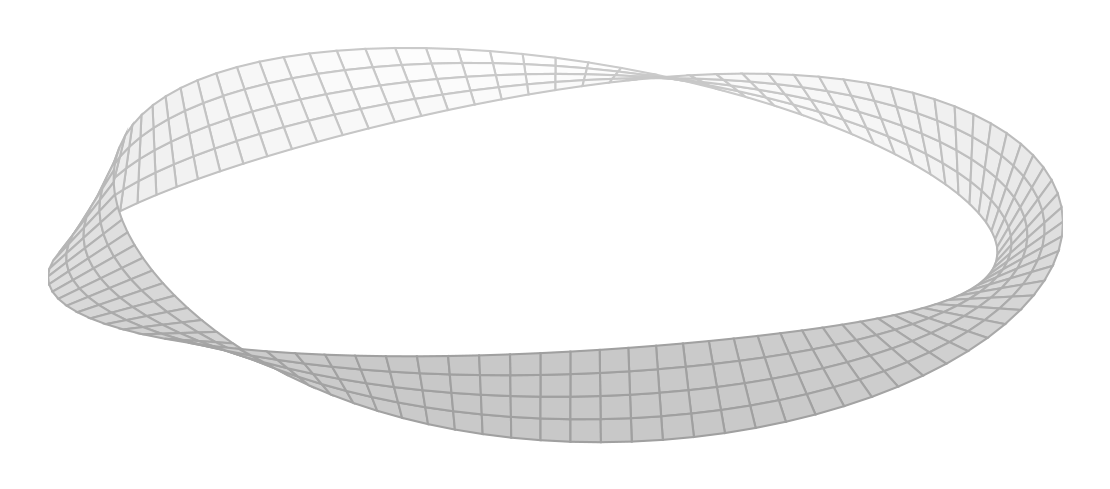
\includegraphics[width=.8\textwidth]{fig/appx/Mobius.png}
    \caption{M\"obius 环}\label{mobius}
\end{figure}

必须指出,用橡皮形变来比喻同胚仍有其局限性。一条纸带不经扭曲,可直接首尾连接得到手环,它具有两个面。扭转半周再相连将得到 M\"obius 环,它只有一个面。扭转一周再相连则又恢复为两个面。这个新环与最初的手环同胚,但却不能通过“揉捏”的方式恢复。如果我们注意到曲面的维度比背景空间的低,而只想关注曲面的内禀性质,则两种手环将视为同⼀空间在 $\R^3$ 内的不同表⽰。所谓的“揉捏”法,实质是 $\R^3$ 的⾃同胚。单看⼆者固然可建⽴同胚,但这种同胚⽆法扩张到整个 $\R^3$ 上。换言之,不存在从 $\R^3$ 的自同胚把两种手环映射在一起,这就解释了问题。这警示我们应更为抽象地看待拓扑。

正如上述例子一样,19 世纪末,人们欲抛掉坐标系而寻求一般集合的拓扑理论。为此要回到同胚的特征:拓扑变化的连续性借助于实数上的 $\epsilon$-$\delta$ 语言,故我们应给出一般集合的连续表述。这一时期可以称为拓扑的分析化,孕育出了\textbf{点集拓扑}。可以说此即最普适的拓扑学。构造这一理论花了很长时间,但我们可简述其关键:极限定义用到了实数集上的小于(序结构)和减法(度量结构),这相当于规定哪类子集是某点邻域、开集和闭集。
因此,拓扑学所研究的对象可以看作脱胎于距离的一种更广义的空间。将这些关键概念抽离出来后,我们就能在拓扑框架下重新得到分析学的定义、命题。现代主流拓扑学正是从这些分析概念出发,一步步走向具象的橡皮几何。
更为深刻的话题将涉及\textbf{代数拓扑}。这一专题将在关于\textbf{上同调}(cohomology)的部分中得以处理,在讨论拓扑分类、积分理论时 de Rham 上同调比较好用。

\section{拓扑空间}

回忆一下,集合 $X$ 的幂集可表示为 $2^X$。$2^X$ 的子集称为\textbf{子集族}(collection of subsets),故全体子集族又构成 $2^{2^X}$。欲对 $X$ 中每个点挑选⼀族⼦集作为其邻域(neighbourhood),即邻域族,就是给定映射 $\mathscr N:X\to 2^{2^X}$ 且 $\mathscr N(x)\ne \mt$。
直观上,邻域只需含有 $x$ 即可,但由于大小任意,可无限接近于 $x$,故有“邻”称。
若 $A\in \mathscr N(x)$,则 $x$ 为 $A$ 的内点(interior point),而 $A$ 中全体内点之集 $A^\circ$ 就是其内部(interior)。

希望从分析学中抽取邻域的若干性质,但不能太多,因为要普适到能包括不同于通常定义的情形。新表述不能依赖距离概念。关键在于,注意属于、包含等集合术语,已能描绘距离所表达的含义:$x$ 在其任意邻域内;$x$ 的任意两邻域之交也是 $x$ 的邻域;$x$ 的任意邻域的内部也是其邻域;包含 $x$ 某邻域的集合也是其邻域。
有了邻域,其它概念都好办了:在某全集 $X$ 下,开集(open set)是满足 $A=A^\circ$ 的集合,闭集(closed set)是其补集为开的集合。因此 $\mt,X$ 是既开又闭的。根据 $\epsilon$-$\delta$ 定义,$f:X\to Y$ 在 $x\in X$ 连续,即 $\forall\epsilon>0$ 都 $\exists\delta>0$,使得 $x$ 的 $\delta$ 邻域的像含于 $f(x)$ 的 $\epsilon$ 邻域。

往往直接考察 $f$ 整体的连续性,但邻域毕竟是就某 $x\in X$ 而言的,可预料从开集出发语言将更优雅。非空开集总是某点的某邻域,而邻域的内部必开,故 $f$ 的连续性表述不必出现邻域概念。有两点考虑:$f$ 不一定是满射,但空集可作为 $Y\backslash\Im f$ 的逆像;$f$ 不一定是单射,满足 $f(z)=f(x)$ 的 $z$ 可以很多,但 $f$ 的连续性要求处处连续,因此 $f(x)$ 任意邻域的逆像一定是所有 $z$ 的某邻域之并。综上,$f$ 连续即 $Y$ 中任意开集之逆是 $X$ 的开集。

由于包含邻域之集也是邻域,因此任意开集之并为开;而两邻域之交为邻域,经由归纳法,只能保证有限个开集之交为开;$\mt,X$ 是开的,$x\in X$ 的邻域则是能包含某个含有 $x$ 的开集的集合。这几条性质显然能导出邻域体系,故为等价表述。

\begin{definition}
$\mathscr{T}\subset 2^X$ 称为 $X$ 的一个\textbf{拓扑}(topology),若:
\begin{itemize}
    \item $\mt,X \in \mathscr{T}$;
    \item $\forall \sigma\subset \mathscr{T}$,$\bigcup_{U\in\sigma} U\in \mathscr{T}$;
    \item $U,V\in\mathscr{T}\To U\cap V\in\mathscr{T}$。或等价地对有限集 $\{A_{i}\} \subset \mathscr{T}$,$\bigcap_{i} A_{i} \in \mathscr{T}$。
\end{itemize}
$\mathscr{T}$ 的元素称为 $X$ 在 $\mathscr{T}$ 下的\textbf{开子集},简称\textbf{开集}。
$(X,\mathscr T)$ 称为 $X$ 关于拓扑 $\mathscr T$ 的\textbf{拓扑空间}。拓扑空间的元素称为\textbf{点}(point)。
\end{definition}

\begin{definition}
    对$x\in X,U\subset X$,若 $\exists O\in\mathscr{T}$ 使 $x\in O\subset U$,则 $U$ 是 $x$ 的一个\textbf{邻域}。$x$ 的全体邻域构成 $\mathscr N(x)$。邻域为开则称\textbf{开邻域},构成 $\mathscr N(x)\cap\mathscr T$。
\end{definition}

\begin{definition}
    $A\subset X$ 称为\textbf{闭集},若 $X\backslash A\in\mathscr{T}$。
\end{definition}

$\mathscr T$ 的名称若自明或不重要,则拓扑空间常略写为$X$。讨论开集时也常省略全集。De Morgan 律指出:并集之补等于补集之交,因此闭集也能给出拓扑的定义。容易得出等价表述为:$\mt,X$ 是闭的;有限闭集之并为闭;任意闭集之交为闭。

拓扑的选取有很多。若 $\mathscr T_1\subset\mathscr T_2$,则称 $\mathscr T_1$ \textbf{较粗}(coarser)或 $\mathscr T_2$ \textbf{较细}(finer)。直观上,较细拓扑容纳更多开集,能区分更多点。\textbf{凝聚}(indiscrete)\textbf{拓扑} $\mathscr T=\{\mt,X\}$ 最粗。\textbf{离散}(discrete)\textbf{拓扑} $\mathscr T= 2^X$ 最细。
分析学中,$\mt$ 和能表为开区间之并的集合都是 $\R$ 上开集,构成 $\R$ 的\textbf{通常}(usual)\textbf{拓扑} $\mathscr T_u$。视 $x,y\in\R$ 的距离为 $|x-y|$,则开区间实质是以 $\frac{x+y}{2}$ 为心的一维球。$(\R,\mathscr T_u)$ 称为\textbf{实直线}。通常拓扑当然比离散、凝聚拓扑更直观,后者一般用于构造反例。

\begin{definition}
    对 $(X,\mathscr T_X),(Y,\mathscr T_Y)$,$f: X \to Y$ \textbf{连续},若 $\forall A\in\mathscr T_Y$,$f^{-1}[A]\in \mathscr T_X$。
\end{definition}

\begin{definition}
    双向连续的双射称作\textbf{同胚}。显然,若空间同胚,则拓扑同势,即开集结构等同。
\end{definition}

\begin{remark}
    同胚的逆也必须连续。考虑复平面上的单位圆周 $C:|z|=1$。按 $f(x)=\e^{\i x}$ 定义 $f:[0,2\pi)\to C$。它是连续双射,但逆不连续。而直观上圆周与区间不能同胚。
\end{remark}

\begin{definition}
置 $(X,\mathscr T)$ 和 $A\subset X$。
\textbf{内部}为开集 $A^\circ:=\bigcup_{O\in\mathscr T\cap 2^A} O$,也即含于 $A$ 的最大开集。
\textbf{闭包}(closure)为闭集 $\bar{A}:=\bigcap_{X\backslash B\in\mathscr T,A\subset B} B$,也即包含 $A$ 的最小闭集。
$\partial A=\bar{A}\backslash A^\circ$ 称为 $A$ 的\textbf{边界}(boundary)。
\end{definition}

\begin{remark}
    显然 $A^\circ\subset A\subset \bar A$。$A^\circ\cup\partial A=\bar A$,$A^\circ\cap\partial A=\mt$。
    
    $\partial A=\mt\iff A^\circ=A=\bar A\iff A$ 既开又闭。
\end{remark}

\begin{theorem}
    $(X\backslash A)^\circ=X\backslash \bar A$。
\end{theorem}
\begin{proof}
    根据定义,$A^\circ:=\bigcup_{X\backslash F\in\mathscr T,X\backslash F\subset A} X\backslash F=X\backslash\bigcap_{X\backslash F\in\mathscr T,X\backslash A\subset F} F=X\backslash\overline{X\backslash A}$。
    替换即可。
\end{proof}

\begin{theorem}
    $A$ 为开集 $\eqto A=A^\circ\eqto\forall x\in A,A\in\mathscr N(x)\eqto\forall x\in A,\exists U\in\mathscr N(x)$ 使 $U\subset A$。
\end{theorem}

\begin{proof}
    $A=A^\circ\in\mathscr T$;反之 $A\in\mathscr T,A\subset A\To A\subset A^\circ\iff A=A^\circ$。

    $A=A^\circ\iff\forall x\in A,\exists O\in\mathscr T$ 使 $x\in O\subset A\iff\forall x\in A, A\in\mathscr N(x)$。
    
    $\forall x\in A$ 下,$\exists U\in\mathscr N(x)$ 使 $U\subset A\To \exists O\in\mathscr T$ 使 $ x\in O\subset U\subset A \To A\in\mathscr N(x)$;反之 $\exists A\in\mathscr N(x)$ 使 $A\subset A$。
\end{proof}

\begin{theorem}
    $A$ 为闭集 $\iff A=\bar A$
\end{theorem}
\begin{proof}
    $A$ 为闭集 $\iff X\backslash A=(X\backslash A)^\circ=X\backslash\bar A\iff A=\bar A$。
\end{proof}

\begin{theorem}
    $x\in\bar A\iff\forall U\in\mathscr N(x),U\cap A\ne\mt$。
\end{theorem}
\begin{proof}
    给定 $x\in\bar A$,假设 $\exists U \in\mathscr N(x),U \cap A=\mt$。则 $\exists O\in\mathscr T$ 使 $x\in O\subset U\To A\subset X \backslash U\subset X \backslash O$,$X \backslash O$ 为闭集 $\To \bar{A} \subset X \backslash O\iff O \cap \bar{A}=\mt$,矛盾;
    给定 $\forall U\in\mathscr N(x),U\cap A\ne\mt$,假设 $x\in X \backslash \bar{A}$。则 $X \backslash \bar{A}\in\mathscr T\To \exists X \backslash \bar{A}\in\mathscr N(x),(X \backslash \bar{A}) \cap A=A \backslash \bar{A}=\mt$,矛盾。
\end{proof}

\begin{definition}
置 $A\subset X$。\textbf{导集}(derived set)为 $A':=\{x \in X:x\in\overline{A\backslash\{x\}}\}$,其元素称为\textbf{聚点}(accumulation point)或\textbf{极限点}。
$\bar{A}=X$ 时称 $A$ 在 $X$ 中\textbf{稠密}(dense)。
\end{definition}
\begin{remark}
    $x\in A'\eqto \forall U\in\mathscr N(x),(U\cap A)\backslash\{x\}=U\cap (A\backslash\{x\})\ne\mt$。$U$ 可等价换为任意含 $x$ 开集。
\end{remark}
\begin{eg}
    考虑实直线,$0,1/2,1$ 都是 $[0,1)$ 的聚点。
\end{eg}

\begin{theorem}
    $\bar A=A\cup A'$。  
\end{theorem}

\begin{proof}
    任给 $x\in A'$。$\forall U\in\mathscr N(x),(U\cap A)\backslash\{x\}\ne\mt\Rightarrow \forall U\in\mathscr N(x),U\cap A\ne\mt\eqto x\in\bar A$。说明 $A'\subset \bar A$,此 $A\cup A'\subset\bar A$;
    任给 $x\in\bar A\backslash A'$。$x\in\bar A,x\notin A'\eqto \exists U\in\mathscr N(x),(U\cap A)\backslash\{x\}=\mt$ 且 $U\cap A\ne\mt\Rightarrow U\cap A=\{x\}\Rightarrow x\in A$。说明 $\bar A\backslash A'\subset A\iff \bar A\subset A\cup A'$。
\end{proof}

\begin{theorem}
    $A$ 为闭 $\iff A'\subset A$。
\end{theorem}
\begin{proof}
    $A$ 为闭 $\iff A=\bar A\iff A=A\cup A'\iff A'\subset A$。
\end{proof}

\begin{definition}
    $S:\N\to X,n\mapsto x_n$ 的值域 $\Im S=\left\{x_n\right\}$ 称为\textbf{序列}或\textbf{点列}。
    若 $\exists x \in X$,$\forall U\in\mathscr N(x),\exists N\in\N$,使 $n>N\To x_n\in U$,则称 $\{x_n\}$ 有\textbf{极限}或\textbf{收敛}于 $x$。
\end{definition}

\begin{remark}
    点列聚点的任意邻域都含点列的无限个点。极限是聚点,但聚点不一定是极限。
\end{remark}

\begin{definition}
    在 $(X,\mathscr T)$ 下,可定义 $A \subset X$ 的\textbf{相对}(relative)\textbf{拓扑}或\textbf{诱导}(induced)\textbf{拓扑} $\mathscr T_r=\{O \cap A: O\in\mathscr T\}$。赋予诱导拓扑的子集称为原集的\textbf{拓扑子空间}(topological subspace)。
\end{definition}

\begin{eg}
    对于实直线和 $A=[0,2]$,在 $\mathscr T_u$ 的诱导下 $B=(1,2]$ 是 $A$ 中的开集。
\end{eg}

\begin{definition}
    给定 $(X,\mathscr T_X),(Y,\mathscr T_Y)$ 和 $Z=X \times Y$。
    定义
    \[\mathscr T_Z=\{O\subset Z:A\in\mathscr T_X,B\in\mathscr T_Y,\text{$O$ 可表为形如 $A\times B$ 的集合之并}\},\]
    $(Z,\mathscr T_Z)$ 称为 $X,Y$ 的\textbf{乘积拓扑空间}(product topological space)。
\end{definition}

这与 $\R$ 的通常拓扑类似,都是通过囊括空集和“任意并”操作来生成拓扑。这一方法可总结如下。取 $\mathscr{B} \subset 2^X$,首先它能覆盖整个 $X$:$\bigcup_{U\in\mathscr{B}}U=X$,其次保持“有限交”性质:对任意有限集 $\{U_i\}\subset\mathscr{B}$,$\exists\mathscr{F}\subset \mathscr{B}$ 使 $\bigcup_{U\in\mathscr{F}}U=\bigcap_{i} U_i$,就称$\mathscr{B}$ 为\textbf{拓扑基}。
$\mathscr{T}=\left\{\bigcup_{U\in\mathscr{F}}U:\mathscr{F}\subset\mathscr{B}\right\}$ 称为 $\mathscr{B}$ 生成的拓扑。\textbf{拓扑子基}的元素所有可能的有限交构成拓扑基。

许多空间往往都难以直接想象或处理,我们可考虑将它分解为简单直观的部分,再重组回去,就能描述复杂的拓扑空间。
设 $\tilde X=\{[x]:x\in X\}$ 是 $(X,\mathscr T)$ 在某个等价关系下的分割或商集(quotient set)。对其规定如下拓扑:映射 $\pi: X \to \tilde X,x\mapsto [x]$ 称为\textbf{自然映射}或\textbf{典范投影},取 $\tilde{\mathscr T}=\{U \subset Y:\pi^{-1}(U)\in\mathscr T\}$,称为\textbf{商拓扑},$(\tilde X,\tilde{\mathscr T})$ 称为\textbf{商空间}。可见,$\pi$ 就好比用来粘合拓扑空间的胶水。
可以证明,设 $\tilde{\mathscr T}^{\prime}$ 为 $\tilde X$ 上另一个拓扑,且使 $\pi$ 连续,则 $\tilde{\mathscr T}^{\prime} \subset \tilde{\mathscr T}$。

\section{度量空间}

我们看到,$\R$ 的距离便可生成一个拓扑基。距离概念的推广自然是在任意集合中,给定满足三角不等式、正定性的对称实函数。开区间也可相应地推广。

\begin{definition}
    \textbf{度量空间}(metric space)是集合 $X$ 和\textbf{距离函数}(或\textbf{度量})$d: X \times X \to [0,\infty)$ 的卡氏积,$\forall x,y,z\in X$ 满足:
    \begin{itemize}
        \item $d(x,y)=d(y,x)$;
        \item $d(x,y) = 0\eqto x=y$;
        \item $d(x,z) \leqslant d(x,y)+d(y,z)$。(三角不等式)
    \end{itemize}
    $B(x,r)=\{y \in X: d(x, y)<r\}$ 称为以 $x \in X$ 为中心、$r$ 为半径的\textbf{开球}(open ball)。
    总可用局部性质构造拓扑:全体开球 $\{B(x,\epsilon):x\in X,\epsilon >0\}$ 就是一个拓扑基,其生成拓扑 $\mathscr T_d$ 就是 $(X,d)$ 的\textbf{度量诱导拓扑},构成 $(X,d,\mathscr T_d)$。称 $(X,\mathscr T_d)$ 是\textbf{可度量的}。
\end{definition}

\begin{remark}
    原则上可以有负定的距离,就像度规一样,但这种距离一般不用于诱导拓扑。
    实际上,具有应用意义的拓扑空间大多都是度量空间。
\end{remark}

\begin{eg}
    \textbf{离散度量}满足 $d_{0}(x,y)=1$ 若 $x \ne y$。这是一个描述离散拓扑的办法。
\end{eg}

\begin{definition}
    置度量空间 $X$。度量 $d_{1},d_{2}$ 是\textbf{等价度量},若 $\exists a,b>0$,使对 $\forall x,y \in X$,有 $a d_{1}(x, y) \leqslant d_{2}(x, y) \leqslant b d_{1}(x, y)$。
\end{definition}

\begin{remark}
    显然等价度量诱导出相同拓扑。
\end{remark}

\begin{eg}
    置 $x=\left(x^1,\cdots,x^{n}\right),y=\left(y^{1},\cdots,y^{n}\right)\in\R^{n}$。$p$-度量为
\[
d_{p}(x, y):=\left(\sum_{k=1}^{n}\left|x^{k}-y^{k}\right|^{p}\right)^{1 / p},\quad p \geqslant 1.
\]
常取$p=2$,称为\textbf{欧氏度量}。
$\R$ 的开球即开区间。$\R^2$ 的开球称为\textbf{开圆盘}。极限为
\[
d_{\infty}(x,y):=\lim_{p\to\infty}d_{p}(x, y)=\max _{1 \leqslant k \leqslant n}\left\{\left|x^{k}-y^{k}\right|\right\}.
\]
任意 $p$-度量等价,诱导出通常拓扑 $\mathscr T_u$。当然,亦可视作 $\R$ 通常拓扑的乘积拓扑。
\end{eg}

我们已悉知 $\epsilon$-$\delta$ 语言可视为连续性在通常拓扑的特例。现在再用度量空间重新叙述。
置 $(X,d_X,\mathscr T_X),(Y,d_Y,\mathscr T_Y)$ 和映射 $f:X\to Y$。$f$ 在 $x \in X$ 处对度量诱导拓扑连续,当且仅当 $\forall\epsilon>0,\exists\delta>0$ 使 $B(x,\delta) \subset f^{-1} [B(f(x),\epsilon)]$。
即 $f^{-1} [B(f(x),\epsilon)]$ 是 $x$ 点邻域。
换言之,$d_X(x,x^{\prime})<\delta\Rightarrow d_Y(f(x),f(x^{\prime}))<\epsilon$。
若 $f$ 在任意点连续,即 $\forall x \in X,\epsilon > 0$,$f^{-1} [B(f(x),\epsilon)]\in\mathscr T_X$,结合“任意并”性质和逆像的保并性,可知 $\forall U\in\mathscr T_Y$,$f^{-1}[U]\in\mathscr T_X$,即 $f$ 连续。

对于度量空间,点列 $\left\{x_n\right\}$ 收敛于 $x$ 等价于 $\lim_{n\to\infty}d(x, x_n)=0$。
点列称为基本列或 Cauchy 列,即$\forall\epsilon>0,\exists N\in\N$使 $k,l>N\Rightarrow d(x_{k},x_{l})<\epsilon$。
度量空间称为\textbf{完备的}(complete),若其中任意 Cauchy 列都收敛于其中的点。实直线上闭区间完备,但开区间不完备:只需注意 $\{1/n\}_{n=2}^\infty$ 在 $(0,1)$ 上无极限。$\R^{n}$ 当然完备。
一致连续性即 $\forall \epsilon>0,\exists\delta>0$ 
使 $\forall x_{1},x_{2} \in X$,$d(x_{1},x_{2})<\delta\Rightarrow d(f(x_{1}),f(x_{2}))<\epsilon$。
注意一致连续要更强:对整个空间要求一致的 $\delta$。

\begin{definition}
    度量空间 $X$ 的子集称为\textbf{有界的},若存在开球包含它。否则称\textbf{无界的}。
\end{definition}

\begin{remark}
    完备性、有界性都不是拓扑不变性。例如,$(0,1)$ 与实直线同胚,但前者不完备、有界,后者完备、无界。
\end{remark}

置度量空间 $X$。$f: X \to X$ 称为(严格)\textbf{压缩映射}(contraction),若 $\exists c\in(0,1)$,使 $\forall x,y \in X$ 且 $x\ne y$,有 $d(f(x),f(y)) \leqslant c d(x,y)$。
仿照分析学可类似证明 \textbf{Banach 不动点定理}:若度量空间 $X$ 完备,$f$ 为一个压缩映射,则 $f(x)=x$ 的解存在且唯一。这是非线性泛函分析的一个有用工具。

\section{紧致性与连通性}

分析学给出了若干等价的实数定理,其中一条是著名的\textbf{Heine-Borel 有限覆盖定理}:若闭区间能被某个开集族覆盖,则可从其中找到有限多元素,构成依旧能覆盖的子族。
19 世纪中叶,Dirichlet 在试图严格化函数连续性时,率先用有限覆盖技术,证明了闭区间上的连续实函数一致连续。
不过他的结果半个世纪后才发表,期间 Heine, Weierstrass 等人各自独立地用类似技术也证明了该结论。Borel 利用这些技术证明了上述的有限覆盖定理。后来 Lebesgue 等人才把它推广到了一般情形。

有限覆盖定理叙述的内容实际上也是一个集合有界闭的充要条件。“有界闭”就是实数闭区间的推广描述。有界性是与距离密切相关的,但有限覆盖性只涉及开集。可见关于有界闭集的分析学命题,很多都能延伸到点集拓扑。

\begin{definition}
    置 $(X,\mathscr T)$。
    $\mathscr C\subset\mathscr T$ 称为 $A\subset X$ 的\textbf{开覆盖}(open cover),若 $A\subset\bigcup_{O\in\mathscr C}O$。
    $\mathscr S\subset\mathscr C$ 是 $\mathscr C$ 的\textbf{子覆盖}(subcover),若它也是开覆盖。若 $\mathscr S$ 是有限集,则称 $\mathscr C$ 存在\textbf{有限子覆盖}。
    $A$ 称为\textbf{紧致的}(compact)或\textbf{紧的},若其任意开覆盖都存在有限子覆盖。
\end{definition}

\begin{eg}
    拓扑基当然是 $X$ 的一个开覆盖。
\end{eg}

\begin{eg}
    实直线上,单点集 $\{x\}\subset X$ 必紧。$\R$、开区间、半开区间非紧。
\end{eg}
\begin{proof}
    对 $\{x\}$ 任取开覆盖 $\mathscr C$,则 $\exists O\in\mathscr C$ 使 $x\in O$,$\{O\}$ 即有限子覆盖。
    不妨以 $(0,1]$ 为例,存在开覆盖 $\{(1/n,2):n\in\N\}$ 不具有限子覆盖;其余情形同理。
\end{proof}

\begin{eg}[Heine-Borel]
    实直线上,闭区间等价于紧集。
\end{eg}

\begin{definition}
    \textbf{仿紧}
\end{definition}


可数公理

\begin{definition}
    \textbf{第二可数}
\end{definition}
给出有用的拓扑结构,使点足够稠密但又不至于太怪异,称为几何背景。

分离公理

\begin{definition}
    拓扑空间 $X$ 称为 $T_2$ 或 \textbf{Hausdorff 的},若对任意不同的两点 $x,y \in X$,存在 $x$ 的开邻域 $A$ 与 $y$ 的开邻域 $B$,使得 $A \cap B=\mt$。
\end{definition}

以拓扑空间为对象、连续映射为态射可构建\textbf{拓扑空间范畴} $\cate{Top}$。

\begin{theorem}
    显然度量空间是 $T_2$ 的。
\end{theorem}

这看起来更像我们所期待的。但是,某些略微非 $T_2$ 的空间会很有用。
\begin{eg}
    在扭量(twistor)理论中。一个“口袋”(pocket)提供了这样的一个例子。考虑实平面的子集 $X$,由实轴上的区间 $[-1,1]$ 和直线 $y=1$ 上的区间 $[0,1]$ 构成,并且等同如下的点:$(x,0) \approx(x,1),0<x \leqslant 1$ 。这样,点 $(0,0)$ 与 $(0,1)$ 就没有不相交的开邻域。严格说来,我们需要下文中商拓扑的概念。
\end{eg}

\begin{eg}
    一个更为地道的非 $T_2$ 空间:考虑正整数组成的空间 $\N_+$,开集取成 $\mt,\N_+$ 以及集合 $\{1,2,3,\cdots,n\}$。这个空间既非 $T_2$ 亦非紧致的(见后面关于紧致的定义)。
\end{eg}

\begin{definition}
    一个拓扑空间 $X$ 称为\textbf{连通的},如果它不能写成两个互不相交 的非空开集的并。有用的两条等价说法是: 任何一个从 $X$ 到赋予离散拓扑的两点集合 $\{0,1\}$ 的连续映射都不是满射;连通拓扑空间只有两个既开又闭的子集。

    给定一拓扑空间 $X$,定义一等价关系如下: $x \sim y$ 当且仅当 $x$ 和 $y$ 属于 $X$ 的 同一个连通子空间。则每个等价类称为 $X$ 的一个\textbf{连通分支}
\end{definition}

\begin{definition}
    设区间 $I\subset\R$ 和拓扑空间 $X$,连续映射 $C:I\to X$ 称为 $X$ 上的一条(有向)\textbf{曲线}(curve)。
    $\sigma\in I$ 称为曲线的\textbf{参数},$\Im C$ 称为\textbf{路径}(path),不混淆时亦可称曲线。
\end{definition}

\begin{definition}
    $C':I'\to $ 称为\textbf{重参数化}。严格单调
\end{definition}

\begin{definition}
    拓扑空间 $X$ 称为\textbf{路径连通的}(path-connected)或\textbf{弧连通的}(arcwise connected),如果 $X$ 中的任意两点都可被一条完全在 $X$ 中的路径连接。
\end{definition}

路径连通的拓扑空间一定是连通的。反之不一定,存在“擦边”的反例。流形的路径连通与连通等价,稍后叙述之。$\R^{n}$ 中的连通开子空间是路径连通的。

列紧性

$\R^{n}$ 中的任何有界序列有一个收敛子列

开球就是连通的

一般总能将非连通集视为有限个连通分支之并,不妨只考虑其中一个连通分支。连通集合称为\textbf{单连通的},就是说,其中任意形似橡皮圈的闭合曲线(称\textbf{简单闭线})所围成的任意曲面都含于此集合中。

单连通区域总同胚开球。

连通区域的表面正是\textbf{闭曲面}。
比如,闭曲面总能将 $\R^n$ 分为有界部分(即所包围区域)和无界部分,因此可区分空间的内外。
一般偏好将法矢取定为朝外,称为\textbf{外指}(outward-pointing)\textbf{法矢},简称\textbf{外法矢}。
单连通的表面就称\textbf{简单闭曲面},简单闭线可视作特殊情形。
物理学总是关注这种良好对象,比如求分段光滑的简单闭曲面的场通量,而实际上分析学的 Gauss 定理的确适用之。
